\documentclass[11pt, oneside]{article} 
\usepackage{geometry}  
\geometry{letterpaper}                   		% ... or a4paper or a5paper or ... 
\usepackage{graphicx}				% Use pdf, png, jpg, or eps§ with pdflatex; use 	
\usepackage{amssymb}
\usepackage{amsmath}
\usepackage[english]{babel}
\usepackage{subcaption}
\usepackage{caption}
\usepackage{float}
\usepackage{natbib}
\graphicspath{{../results/}}

%SetFonts

%SetFonts


\title{MiniProject - Comparison between different models applied on biological population growth}


\author{Xuan Wang (xuan.wang22@imperial.ac.uk)}


\date{2 Dec, 2022}					

\footnotetext[1]{Word Count:}

\linespread{1.5}

\begin{document}
\nocite{*}
	\maketitle
	\newpage

	\begin{abstract}
% background/objectives/methods/main results/main conclusions/take-home messages
	Due to the availability of 
	\end{abstract}
	\pagebreak

	\section{Introduction}

	For decades, great attention has been paid to microbial population growth, and many studies have been conducted in this area. The impact of bacterial population growth rate on the safety of food products is one of the major reasons attracting researchers to study in this field, such that effective intervention could be given to the production process with valuable and accurate prediction \cite{Nauta}. With the increasing interest in microbial growth, the suitability of models has become a popular topic due to their importance in bringing considerable savings caused by the challenge in laboratory testing \cite{perni2005estimating}. 
	\bigbreak
	\noindent In general, bacterial growth contains several stages: the lag phase, exponential phase, stationary phase, and death phase \cite{doi:10.1080/10408398.2011.570463}. Several models have been developed for the evaluation, including phenomenological models - developed based on experimentally observed patterns instead of any basic principles; and another type called the mechanistic microbial growth model - which takes the theories into consideration \cite{doi:10.1080/10408398.2011.570463}. The objective of our study is to investigate the overall performance of different models applying to the microbial growth rate data across species. To achieve this, the quadratic and cubic linear polynomial models are selected as representative models for the phenomenological models. A comparison with the linear models will be given to the Logistic model, the modified Gompertz model, and the Baranyi model, which are regarded as mechanistic models. In addition to the non-linear models, the linear polynomial models will also be included in our study for comparison. The non-linear Least Squares approach is used for our study due to the more negligible bias for the non-linear models. 
	\bigbreak
	\noindent This report will be divided into several parts:
	\begin{itemize}
	\item Methods
	\\This section will include an overall description of the methods used in this study, including the process of the data, the expressions of the models used, the method for model fitting and the computing tools used to reproduce the procedure.
	\item Results
	\\The diagrams of the models and the results of the model selection will be displayed in this section. A brief interpretation will be given along with the graphs.
	\item Discussion
	\\The discussion will include the analysis of the results section and the implication to reality with a combination of several previous literatures. The gaps for future work to cover will also be mentioned at the end of the discussion section.
	\item Conclusion
	\\The key findings of this study will be summarised in this section.
	\end{itemize}

	\pagebreak

	\section{Methods}


	For a comprehensive comparison, this report uses a combination of the Ordinary Linear and Non-Linear Least Squares (NLLS) approaches, which are applied to the linear and non-linear models, respectively. Each model is fitted to the given dataset separately, and the models are compared by superimposing the plots in one graph. For the model selection, both the Akaike Information Criterion (AIC) and Bayesian Information Criterion (BIC) are calculated. It is also worth mentioning that, though the \(R^2\) has been a popular method for evaluating model fitness, it will not be used for this study. The reason is that the calculation of \(R^2\) value could provide high bias when estimating non-linear models \cite{spiess2010evaluation}, while AIC and BIC have a better performance in this situation. Therefore, AIC and BIC are performed in our study for the selection of models instead.

 		\subsection{Data}
 
		The dataset used for this analysis includes the measurement of change in biomass or the number of cells of microbes over time, the corresponding temperature, measurement units, etc. The primary data from the dataset consists of the population and time, where time is used as the independent variable and population as the dependent variable. In this study, we assume that all the other potential factors for the population are held constant. Considering the non-negativeness of the data in reality, the absolute values of raw data for time and abundance are used to avoid misleading results. In addition, for a precise analysis of the dataset across different species, the dataset is divided into multiple subsets identified by the unique combination of temperature, species, medium, citation and replicate. 285 subsets are generated representing different groups. Due to the restriction of the modified Gompertz model, which requires the logarithm form of data, the abundance data is transformed for all non-linear modellings in this paper for a more explicit comparison. Though the original data is required for fitting linear models, the results will be converted to a logarithm form for comparison. The log-transformed data is used for non-linear models.

 		\subsection{Models}
 
 		To start with, the linear models are performed.  As the most commonly seen models for bacterial growth, the Logistic model and the Gompertz models are conducted for comparison. In addition, as a mechanistic model, the Baranyi model is also shown in this study.
		
			\subsubsection{The Linear models}
			
			The simplicity and broad usage of linear polynomial models have been the major advantages. The empirical expression of the linear models used are:
			\[y = ax^2 + bx + c\]
			\[y = ax^3 + bx^2 + cx + d\]
			\noindent Here \(a, b, c, d\) are all parameters to be determined by modelling. Both quadratic and cubic linear models are employed for our comparison to ensure that the result is reliable. Since the bacterial population growth contains several phases, the unitary linear model would cause great bias and therefore is not applied in our study.
			
 			\subsubsection{The Logistic model}
			
			As a more widely-fitting choice, the non-linear models are generally more robust than linear models for prediction \cite{Archontolis}. Among these models, the Logistic model has been a classical choice for prediction in biological population. This model can be expressed as follows:
			
			\[N_t = \frac{N_0 N_{max} e^{rt}}{N_{max} + N_0(e_{rt} - 1)}\]
			
			\bigbreak
			\noindent In this expression, \(N_t\) represents the population size at time \(t\), \(N_0\) is the initial population size, \(N_{max}\) is the maximum carrying capacity, and the \(r\) is the growth rate of the population. 
			
			\subsubsection{The modified Gompertz model}
			
			Though the simplicity of the Logistic model has been an advantage, the formula does not contain the time lag before the start of exponential growth in bacterial population growth. In reality, the existence of lag phase is common in biology, which allows the bacterial cells to adapt to the new environment \cite{rolfe2012lag}. This shortage of Logistic model could be solved by the modified Gompertz model \cite{zwietering1991modeling}(Zwitering et al., 1990), which has the following formula:
			
			\[log(N_t) = N_0 + (N_{max} - N_0) e^{-e^{r_{max}exp(1)\frac{t_{lag}-t}{(N_{max}-N_0)log(10)} + 1}}\]
			
			\bigbreak
			\noindent Similar to the Logistic model, the parameter \(N_t\) is the bacterial population size at time \(t\), and \(N_0\) is the initial one; \(r_{max}\) is the maximum growth rate of bacterial growth, which can be generated by calculating the tangent to the inflection point; \(t_{lag}\) is the duration of the lag phase.
			
			\subsubsection{The Baranyi model}
			
			In addition to the Gompertz model, the lag phase of population growth is also taken into consideration by the Baranyi model. The Baranyi model is also examined in our study with the explicit expression \cite{BARANYI1994277}:
			\[N_t = N_0 + r_{max} A(t) - \frac{1}{m}ln(1 + \frac{e^{mr_{max}A(t)} - 1}{e^{m(N_{max} - N_0)}})\]
			where
			\[A(t) = t + \frac{1}{r_{max}}ln(e^{-vt} + e^{-h_0} - e^{-vt - h_0}) \]
			\begin{itemize}
			\item \(N(t) = ln(x(t))\), where \(x(t)\) is the cell concentration at time \(t\) with unit \(\frac{CFU}{ml}\);
			\item \(r_{max}\) is the maximum growth rate;
			\item \(m\) is a curvature parameter to characterise the transition from the exponential phase;
			\item \(v\) is a curvature parameter to characterise the transition to the exponential phase;
			\item \(h_0\) is a dimensionless parameter that quantifies the cells' initial physiological state. \cite{GRIJSPEERDT1999593}
			\end{itemize}
			\noindent According to Baranyi (1997), it is suggested that \(v = r_{max}\) and \(m = 1\), which will also be adopted for our study \cite{GRIJSPEERDT1999593}. It is also mentioned that the parameter \(h_0\) could be derived by the production of \(r_{max}\) and \(t_{lag}\)\cite{BARANYI1994277}. 
			
 		\subsection{Model fitting}
		
		The computation of linear modelling can be achieved in R directly by using the \(lm()\) function, which could realise both quadratic and cubic modelling. As mentioned, the data used in the model fitting of both linear models are the raw data instead of log-transformed data. For the non-linear models, the logarithm form of the population data is used for the fittings. The starting values are defined with the same equation within a loop for each subset, which takes the value of \(N_0\) as the minimum value of population in each subset while \(N_{max}\) takes the maximum value; for the maximum growth rate, the value of \(r_max\) is obtained by taking the maximum slope value between every two points of the data; the location of the maximum growth rate is used to derive the start value of the duration of the lag phase by subtracting the time duration of the exponential growth phase from the overall time. For the model selection criterion, we have used both AIC and BIC, while the formula of AIC differs when the sample size is small to ensure that the comparison result is reliable. The expressions of the selection criterion are as follows:
		
		\[AIC = n + 2 + nlog(\frac{2\pi}{n}) + nlog(RSS) + 2p\]
		\[BIC = n + 2 + nlog(\frac{2\pi}{n}) + nlog(RSS) + plog(n)\]
		For small samples:
		\[AIC' = AIC + \frac{2p(p + 1)}{n - p - 1}\]
		
		\noindent In the expression, RSS refers to Regression Sum of Squares (RSS); n represents the sample size; p is the number of parameters in the corresponding model.

 		\subsection{Computing tools}
		Both Python and R have been used for our study. Specifically, Python is used for data processing, which includes transforming raw data to absolute value and identifying unique growth rates. This is due to the powerful Python data-processing packages, including \(panda\), which is helpful to the initial inspection and process of raw data for analysis. R is used for the following steps, including model fitting and graph plotting, due to the convenience of data visualisation with the use of packages such as \(ggplot2\). In addition, a shell script is included for running the entire project, including this report. \\
		\\
		For the full run of the scripts, the following packages need to be installed: 
 	\bigbreak
 	\noindent \(R:\)
 	\begin{itemize}
	\item \(ggplot2\) - This package is used for the plotting of graphs, including the model plots and the AIC/BIC comparison plots;
	\item \(stats\) - The \(lm()\) function in \(stats\) package is used for the linear model fittings;
	\item \(minpack.lm\) - The non-linear model fitting process employed the function of \(nlsLM()\) function in this package, which uses the Levenberg-Marqualdt algorithm instead of the Gauss-Newton algorithm in \(nls\) function. The advantage of this algorithm is that a wider range of starting values could be accepted without running into an error compared to \(nls\) function;
	\end{itemize}
	\(Python:\)
	\begin{itemize}
	\item \(pandas\) - Used to read the dataset.
	\end{itemize}
		\pagebreak
	\section{Results}
	
		In this section, the results generated from our modelling will be displayed and interpreted. To solve the general question about how well different mathematical models fit data across species, selected results that could be considered representative among the total 285 subsets will be shown. The spots in the plots represent the original data point, and the superimposed lines stand for the models fitted. To ensure the comprehensiveness of the comparison, the displayed figures will include the following categories:
		\begin{itemize}
		\item General patterns with death phase
		\item General patterns with exponential growth phase and stationary phase
		\item Groups with a significant lag phase
		\item Groups with different sample deviation
		\item Groups with different sample sizes
		\end{itemize}
		
		\subsection{Plottings}

		\begin{figure}[H]
			\begin{center}
			\begin{minipage}{.5\textwidth}
				\centering
				\includegraphics[page=4, scale = 0.5]{plot_subsets.pdf}
			\end{minipage}%
			\begin{minipage}{.5\textwidth}
				\centering
				\includegraphics[page=66, scale = 0.5]{plot_subsets.pdf}
			\end{minipage}
			\end{center}
		\caption{General patthern with death phase}
		\end{figure}
		
		\noindent As shown above, Figure 1 displays the general pattern of two subsets with the death phase counted. In the graphs, both linear models showed a pattern of decline at the end, while the Logistic and Gompertz models remained almost constant when the original data was reduced. By contrast, the Baranyi model shows a better sensitivity to the reduction, though deviation is observed from the actual data value. 
				
		\begin{figure}[H]
			\begin{center}
			\begin{minipage}{.5\textwidth}
				\centering
				\includegraphics[page=41, scale = 0.5]{plot_subsets.pdf}
			\end{minipage}%
			\begin{minipage}{.5\textwidth}
				\centering
				\includegraphics[page=90, scale = 0.5]{plot_subsets.pdf}
			\end{minipage}
			\end{center}
		\caption{General pattern with exponential growth phase and stationary phase}
		\end{figure}
		
		\noindent From this figure, it is noticeable that though the Baranyi model fits better than the other two non-linear models for the death phase, the modified Gompertz and Logistic models do a better job for the modelling of the stationary phase. Fluctuations are shown by the Baranyi model in the stationary phase, which deviates from the original point. No significant difference was observed in the models' performance in the exponential growth phase in the second graph.
		
		\begin{figure}[H]
			\begin{center}
			\begin{minipage}{.5\textwidth}
				\centering
				\includegraphics[page=89, scale = 0.5]{plot_subsets.pdf}
			\end{minipage}%
			\begin{minipage}{.5\textwidth}
				\centering
				\includegraphics[page=65, scale = 0.5]{plot_subsets.pdf}
			\end{minipage}
			\end{center}
		\caption{Pattern with different sample deviation}
		\end{figure}
		
		\noindent The figure above displays the comparison of the model fittings in samples with different standard deviations. The samples show a more significant divergence in the first image, especially at the starting period. It can be observed that the line for the Baranyi model is not present in the first graph, which indicates that the model cannot fit this subset with a more significant standard deviation. By contrast, the other chosen models fit the subsets well without any obvious difference in the figure. However, it is also worth mentioning that the linear models have a better performance in the second image with a minor standard deviation, even though the difference is relatively small.
		
		\begin{figure}[H]
			\begin{center}
			\begin{minipage}{.5\textwidth}
				\centering
				\includegraphics[page=178, scale = 0.5]{plot_subsets.pdf}
			\end{minipage}%
			\begin{minipage}{.5\textwidth}
				\centering
				\includegraphics[page=118, scale = 0.5]{plot_subsets.pdf}
			\end{minipage}
			\end{center}
		\caption{Pattern with significant lag phase}
		\end{figure}
		
		\noindent As displayed in figure 4, we can notice that the most significant advantage of non-linear models is the sensitivity of lag phases compared to linear models. The Baranyi and Gompertz models show a similar fit in the first image, while the linear and Logistic models fail to fit the lag phase. The second graph shows a slight difference, where the Baranyi model shows worse evaluation than the Logistic model. The modified Gompertz model estimates the lag phase best from our results.

		\begin{figure}[H]
			\begin{center}
			\begin{minipage}{.5\textwidth}
				\centering
				\includegraphics[page=56, scale = 0.5]{plot_subsets.pdf}
			\end{minipage}%
			\begin{minipage}{.5\textwidth}
				\centering
				\includegraphics[page=285, scale = 0.5]{plot_subsets.pdf}
			\end{minipage}
			\end{center}
		\caption{Pattern with different sample size}
		\end{figure}
		
		\noindent Figure 5 compares the model fittings for samples with different sizes. It is noticeable that the larger sample size would lead to a better estimate of the Gompertz and the Logistic model, while the Baranyi model again fails to fit the sample with a large sample size. In addition, the linear models have a comparatively more deviated estimation in the second image. Errors can be observed from the linear models in the second graph in the growth phase.
		
		\begin{figure}[H]
			\begin{center}
			\begin{minipage}{.5\textwidth}
				\centering
				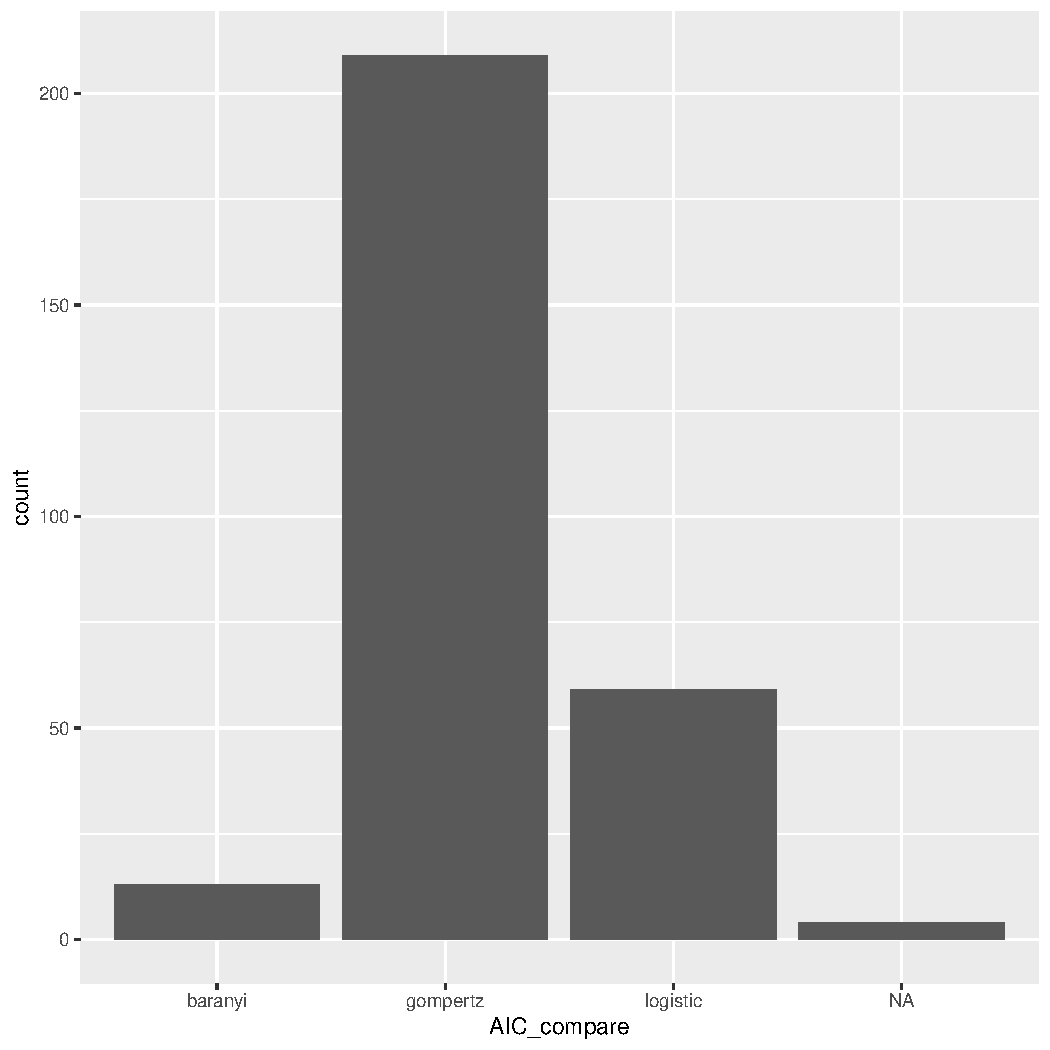
\includegraphics[scale = 0.4]{AIC_plot.pdf}
			\end{minipage}%
			\begin{minipage}{.5\textwidth}
				\centering
				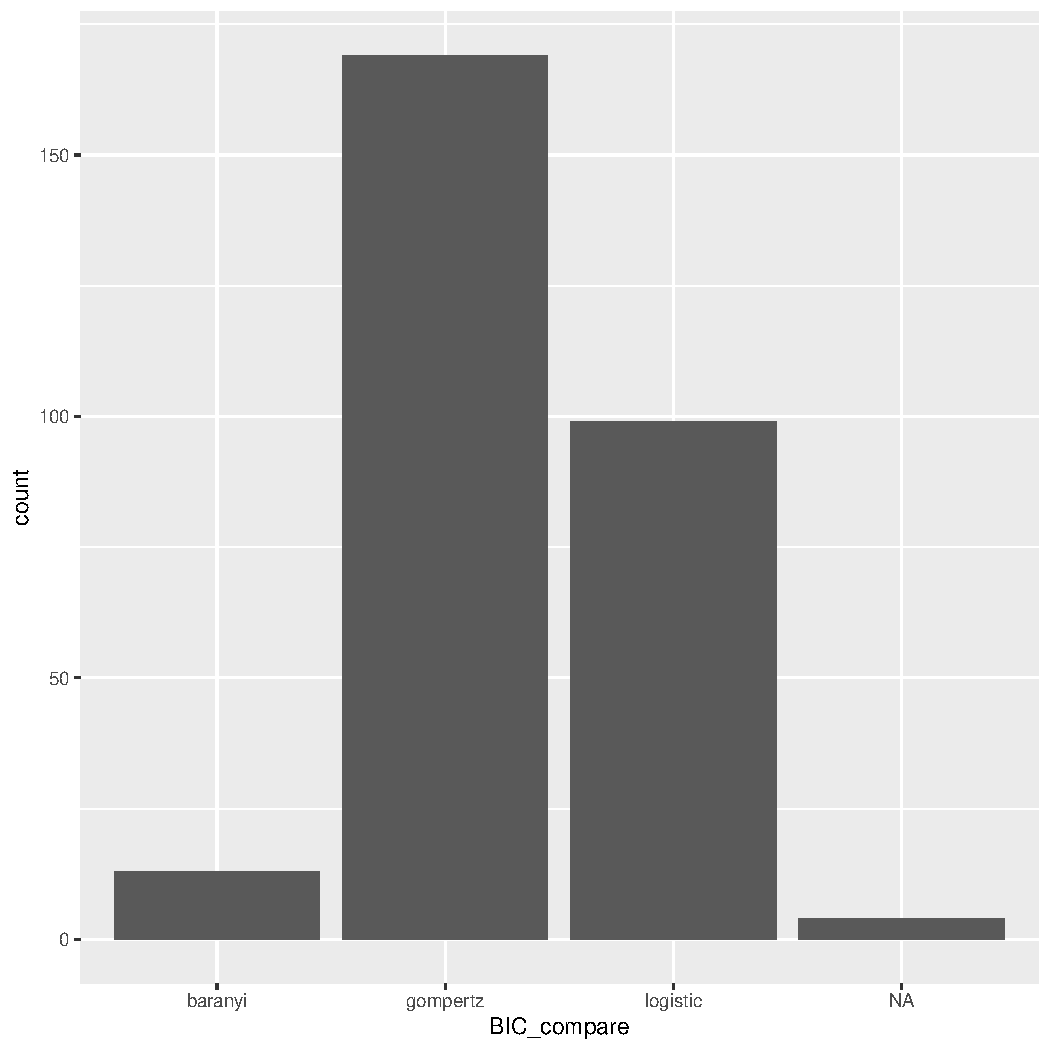
\includegraphics[scale = 0.4]{BIC_plot.pdf}
			\end{minipage}
			\end{center}
		\caption{AIC and BIC comparison}
		\end{figure}
		
		\noindent Now we proceed to the numerical comparison using the AIC and BIC calculation. It can be seen that both criteria have shown similar results, with the Gompertz model having the highest frequency of minimum AIC/BIC value among all the chosen models. Meanwhile, though the linear models are also included,  there is zero frequency of linear models having the lowest value. Therefore, we can conclude that the non-linear models fit data better than linear models in general, with the Gompertz model providing the best estimation.

	\pagebreak
	\section{Discussion}
	
	\subsection{Findings and implications}
	
	As indicated by the results above, the performance of Quadratic and Cubic linear models usually cannot predict the whole trend in general. Although the linear models perform better in predicting the death phase, their overall AIC and BIC are higher than others. This could be because bacterial growth could usually be affected by various factors which may not be captured in the pure mathematical functions \cite{sutherland2002behavioural}. For example, both linear models miss the lag phase before the start of population growth. This is because the phenomenological models usually do not consider the lag time. Nevertheless, the existence of the lag phase is proven in reality \cite{rolfe2012lag}, causing inaccuracy of linear models. By contrast, this is usually taken into account by the mechanistic models, which are based on biological theory, hence providing better performance on predicting the lag phase. Though the fitting of the Baranyi model for the lag phase shows a slight deviation in the second plot of figure 4, it could be due to several reasons:
	\begin{itemize}
	\item The current studies on the lag phase are still not sufficient enough \cite{rolfe2012lag}. Due to the lack of data on the underlying biological behaviour and physiological processes, current studies on the lag phase is still poor. This could be a potential reason for the shortage of theoretical-based models when predicting the duration before the start of exponential growth.
	\item Another possible reason is the limited sample data for the lag phase. According to Schmidt, the actual lag time has to be determined from the laboratory data instead of the model \cite{Ylmaz2011IdentifiabilityOB}. Nevertheless, there are only a few points at the lag phase in our dataset, which could be a possible reason for an inaccurate estimate of the model.
	\end{itemize}
	\noindent For the estimate of the stationary phase, the performance of models is relatively close. In general, most models provide a reasonable pattern for the stationary duration, while some error is displayed in the Baranyi model. There are fluctuations shown in the Baranyi model even when the abundance becomes stable. In this situation, the linear models perform better, while the Gompertz and Logistic models can also provide an accurate estimation. It is hard to distinguish which model has the best estimate at the stationary stage.
	\bigbreak
	\noindent It is worth mentioning that one advantage of the phenomenological models is their better ability to predict the death phase compared to the Gompertz and Logistic models. Although the Baranyi model also considers the estimation of the death phase, the overall fitness is not satisfying. The Gompertz and Logistic model reaches the maximum and stays almost constant without extending beyond the stationary phase \cite{whiting1992quantitative}. This may be due to the empirical nature of these model equations, where the death phase is not taken into account \cite{chowdhury2007validity}. By comparison, both quadratic and cubic equations can provide an accurate estimate for the decline of abundance after stationarity, according to our results. The original nature of the mathematical equations could be an explanation, which contains both an increase and reduction in a period. We can conclude that the equations based on pure mathematical theories can sometimes also be helpful, despite the specific situation which may not be suitable for every case. Though the mechanistic models generally provide a better estimate, the fitness depends on the different parameters taken into account. 
	\bigbreak
	\noindent In addition, it is noticeable that the sample size and the standard deviation are also factors that could influence the performance of models. We observe that the Baranyi model was not included in the graph for the larger sample size and standard deviation in both Figure 3 and Figure 5. This is due to the model's poor fit in the corresponding subset. It can be concluded that the range of datasets that the Baranyi model can fit is comparatively smaller than the other models. All the other chosen models have a reasonable fit for the data with different standard deviations. In contrast, the linear models show an inaccuracy for the estimation of the dataset with a greater sample size. 
	\bigbreak
	\noindent In general, we can conclude that the overall performance of the modified Gompertz model has the best estimation for our dataset. Mechanistic models based on biological theories can usually provide a better estimate than phenomenological ones, with the parameters counted being a critical factor of the effectiveness and comprehensiveness of the mechanistic model. 
	
	\subsection{Shortcomings}
	
	Though several models have been conducted for our study, it is not comprehensive enough, and further work still needs to be done to cover the gap. There are several shortcomings of this study:
	\begin{itemize}
	\item Changes in the environment not taken into account
	\bigbreak
	\noindent Though it is possible to predict the population growth rate, the environment is still likely to alter, which could bring unexpected change in population \cite{sutherland2002behavioural}. For example, several factors could potentially influence bacterial growth, including temperature, pH value, etc. \cite{gale1943factors} However, the change of environment could cause uncertainties during the data collection process, which might not be included in the data. This would be a potential cause for the deviation of the modelling, and could lead to different results in the model performances.
	\item Possible inaccuracy by the data processing
	\bigbreak 
	\noindent In this study, the raw data of the cell population and time are transformed to their absolute value for further calculation to ensure that the data is realistic. However, it is possible to misunderstand the data with negative values at their initial state.
	\bigbreak
	\item Difference in the definition of parameters
	\noindent According to the study of \cite{perni2005estimating}, the definition of the parameters are usually determinant to the suitability of the models. In our study, the models are all compared with the same starting point to ensure that they all have the same standard. However, some parameters could slightly differ from other models, which is not considered in our study. This could also be a potential cause for inaccuracy, and further studies need to be conducted.
	\end{itemize}
	
	\section{Conclusion}
	
	In this study, we have applied the Baranyi model, the modified Gompertz model and the Logistic model with comparison to the Quadratic and the Cubic linear model to find the model of the best estimate for the functional response data across different species. The results have suggested that the modified Gompertz model has the best performance in general, even though the death phase estimation is not considered. Despite the observation that the phenomenological models could be effective when providing prediction after exponential growth due to mathematical properties, the models based on population growth theories are more suitable for the overall estimates, where the parameters taken into account should be a primary factor influencing the effectiveness of the models.
	\pagebreak

\bibliographystyle{agsm}
\bibliography{report}
\end{document}  